\section{Explanation Factors}
    \indent 
    In this part, we take a look at explanation factors from two studies and try to find requirements for successful explanations. The first research suggests a standard way to evaluate explanations while the second study aims at designing explanations.
    
    \subsection{The first framework - Seven Explanatory criteria}

        \indent 
        Like what we have already mentioned in the second part, literature review, which the ``seven explanatory criterion'' \cite{tintarev2007survey}(see table \ref{table:1}) from Nava Tintarev and Judith Masthoff is the most popular standard used to evaluate the explanation. It is comprehensive since it summarized all advantages which explanation can bring to the system.

        \begin{table}[ht] 
            % ht used to attach the table to the position approximately where they are wrote here
            \centering
            \begin{tabular}{ | m{8em} | m{4cm} | }
            \hline
            %  \bfseries used to bold the header
            \bfseries Aim & \bfseries Definition\\ [0.5ex] 
            \hline\hline
            Transparency & Explain how the system works\\ 
            \hline
            Scrutability & Allow users to tell the system it is wrong\\ 
            \hline
            Trust & Increase users' confidence in the system\\ 
            \hline
            Effectiveness & Help users make good decisions\\ 
            \hline
            Persuasiveness & Convince users to try\\ 
            \hline
            Efficiency & Help users make decisions faster\\ 
            \hline
            Satisfaction & Increase the ease of use or enjoyment\\ 
            \hline
            \end{tabular}
            \caption{Explanatory criteria and their definitions}
            \label{table:1}
        \end{table}

        \indent 
        Although they may have different names in different studies (``explanation attributes'' \cite{al2013explanations}, ``seven possible aims for explanations'' \cite{tintarev2012evaluating} or ``quality factors'' \cite{gedikli2014should}). The basic idea is the same, that is to make a recommender system more understandable by users.
        
        \indent 
        \textbf{\textit{Transparency:}} Transparency in a recommender system is related to the capability of a system to expose the reasoning behind a recommendation to its users \cite{herlocker2000explaining}. A recommender system without explanation works like a ``black box'', which may lose users' trust. Thus, transparency is considered as an important factor to build user's trust in a recommender system \cite{swearingen2002interaction}.

        \indent 
        \textbf{\textit{Scrutability:}} Scrutability means, in short, allow users to tell the system it is wrong. It can also be seen as a kind of User Control, which allows users to correct reasoning from system \cite{czarkowski2002scrutable}.

        \indent
        \textbf{\textit{Trust:}} Trust is sometimes linked with transparency. Studies have already shown that transparency and the possibility of interaction with recommender systems increase user trust \cite{felfernig2007knowledge} \cite{sinha2002role}.

        \indent
        \textbf{\textit{Effectiveness:}} An effective explanation can help users to make a better decision. If an item suggested by the system is the one the user likes, such an explanation can be considered as effective.

        \indent
        \textbf{\textit{Persuasiveness:}} Persuasiveness, sometimes referred as promotion, is strongly related to effectiveness and can be defined as the ability of an explanation type to convince the user to accept or disregard certain items \cite{gedikli2014should}.

        \indent 
        \textbf{\textit{Efficiency:}} An explanation is usually considered as efficient when it helps the user to decide more quickly or when it helps to reduce the cognitive effort required in the decision process \cite{gedikli2014should}. The most common approach to measure it is to look at the interaction time between users and the recommender system.

        \indent 
        \textbf{\textit{Satisfaction:}} The user’s overall satisfaction with a recommender system is assumed to be strongly related to the perceived quality of its recommendations and explanations \cite{swearingen2002interaction}.

        \indent 
        What we need to bear in mind, is that it is hard to design an explanation which obeys all of these seven criteria. In most of the time, we need to have a trade-off. For instance, an explanation that offers good transparency may impede efficiency as the user may spend more time in reading the explanations \cite{tintarev2007survey}.
        In reality, the choice of criteria depends on the goal of the system. 

\subsection{The second framework Question-type-based Explanation}

    \indent
    Another possible way to evaluate and design explanations in context-aware applications is to focus on different question types. Lim et al. have proposed eight question-type-based explanations \cite{lim2010toolkit}.

    \indent These eight question types are:

    \begin{enumerate}
        \item \textbf{\textit{Input:}} Explanations inform users which information sources are used to generate the recommendation.
        \item \textbf{\textit{Output:}} Explanations inform users which output/result is generated by the system.
        \item \textbf{\textit{What:}} System explains the current state to users (what it is now).
        \item \textbf{\textit{What If:}} Which results will be generated, if users alter his/her input values(change the behavior).
        \item \textbf{\textit{Why:}} Explanations inform users why the application derived its output value from the current (or previous) input values\cite{lim2010toolkit}.
        \item \textbf{\textit{Why Not:}} Explanations inform users why another output/result is not chose.
        \item \textbf{\textit{How to:}} Explanations tell users what they can do so that they can get another output/result.
        \item \textbf{\textit{Certainty:}} Explanations tell users, how certain/uncertain the output/result is.
    \end{enumerate}

    \indent Although the original use case of eight questions is a context-aware application, we can find explanations from other recommender systems which also apply these principles. For example, an e-commercial website which tells you that your recommendations are based on your purchase record. This kind of explanation can be seen as a Why-type-question.  The next section will show a more detailed example.
    
    \subsection{Example -- Explanations in Google Advertisement Recommendation Service}
        \indent In this section, we apply both of the frameworks introduced above with a real-world use case.  We try to illustrate how these explanation principles work with a personalised online advertisement service.

        \indent Users see nowadays more and more frequently online advertisement when they browser on the Internet. For example, Google Search results page may show ads similar to a search keyword the user just typed. It is a kind of personalised service provided by Google since every user may get their customised results, in other words, see different advertisements \cite{googleAdSetting}. 
        
        Figure \ref{img:googleAd1} shows an example of Google Ads.
        \begin{figure}[H]
            \centering
            \captionsetup{justification=centering}
            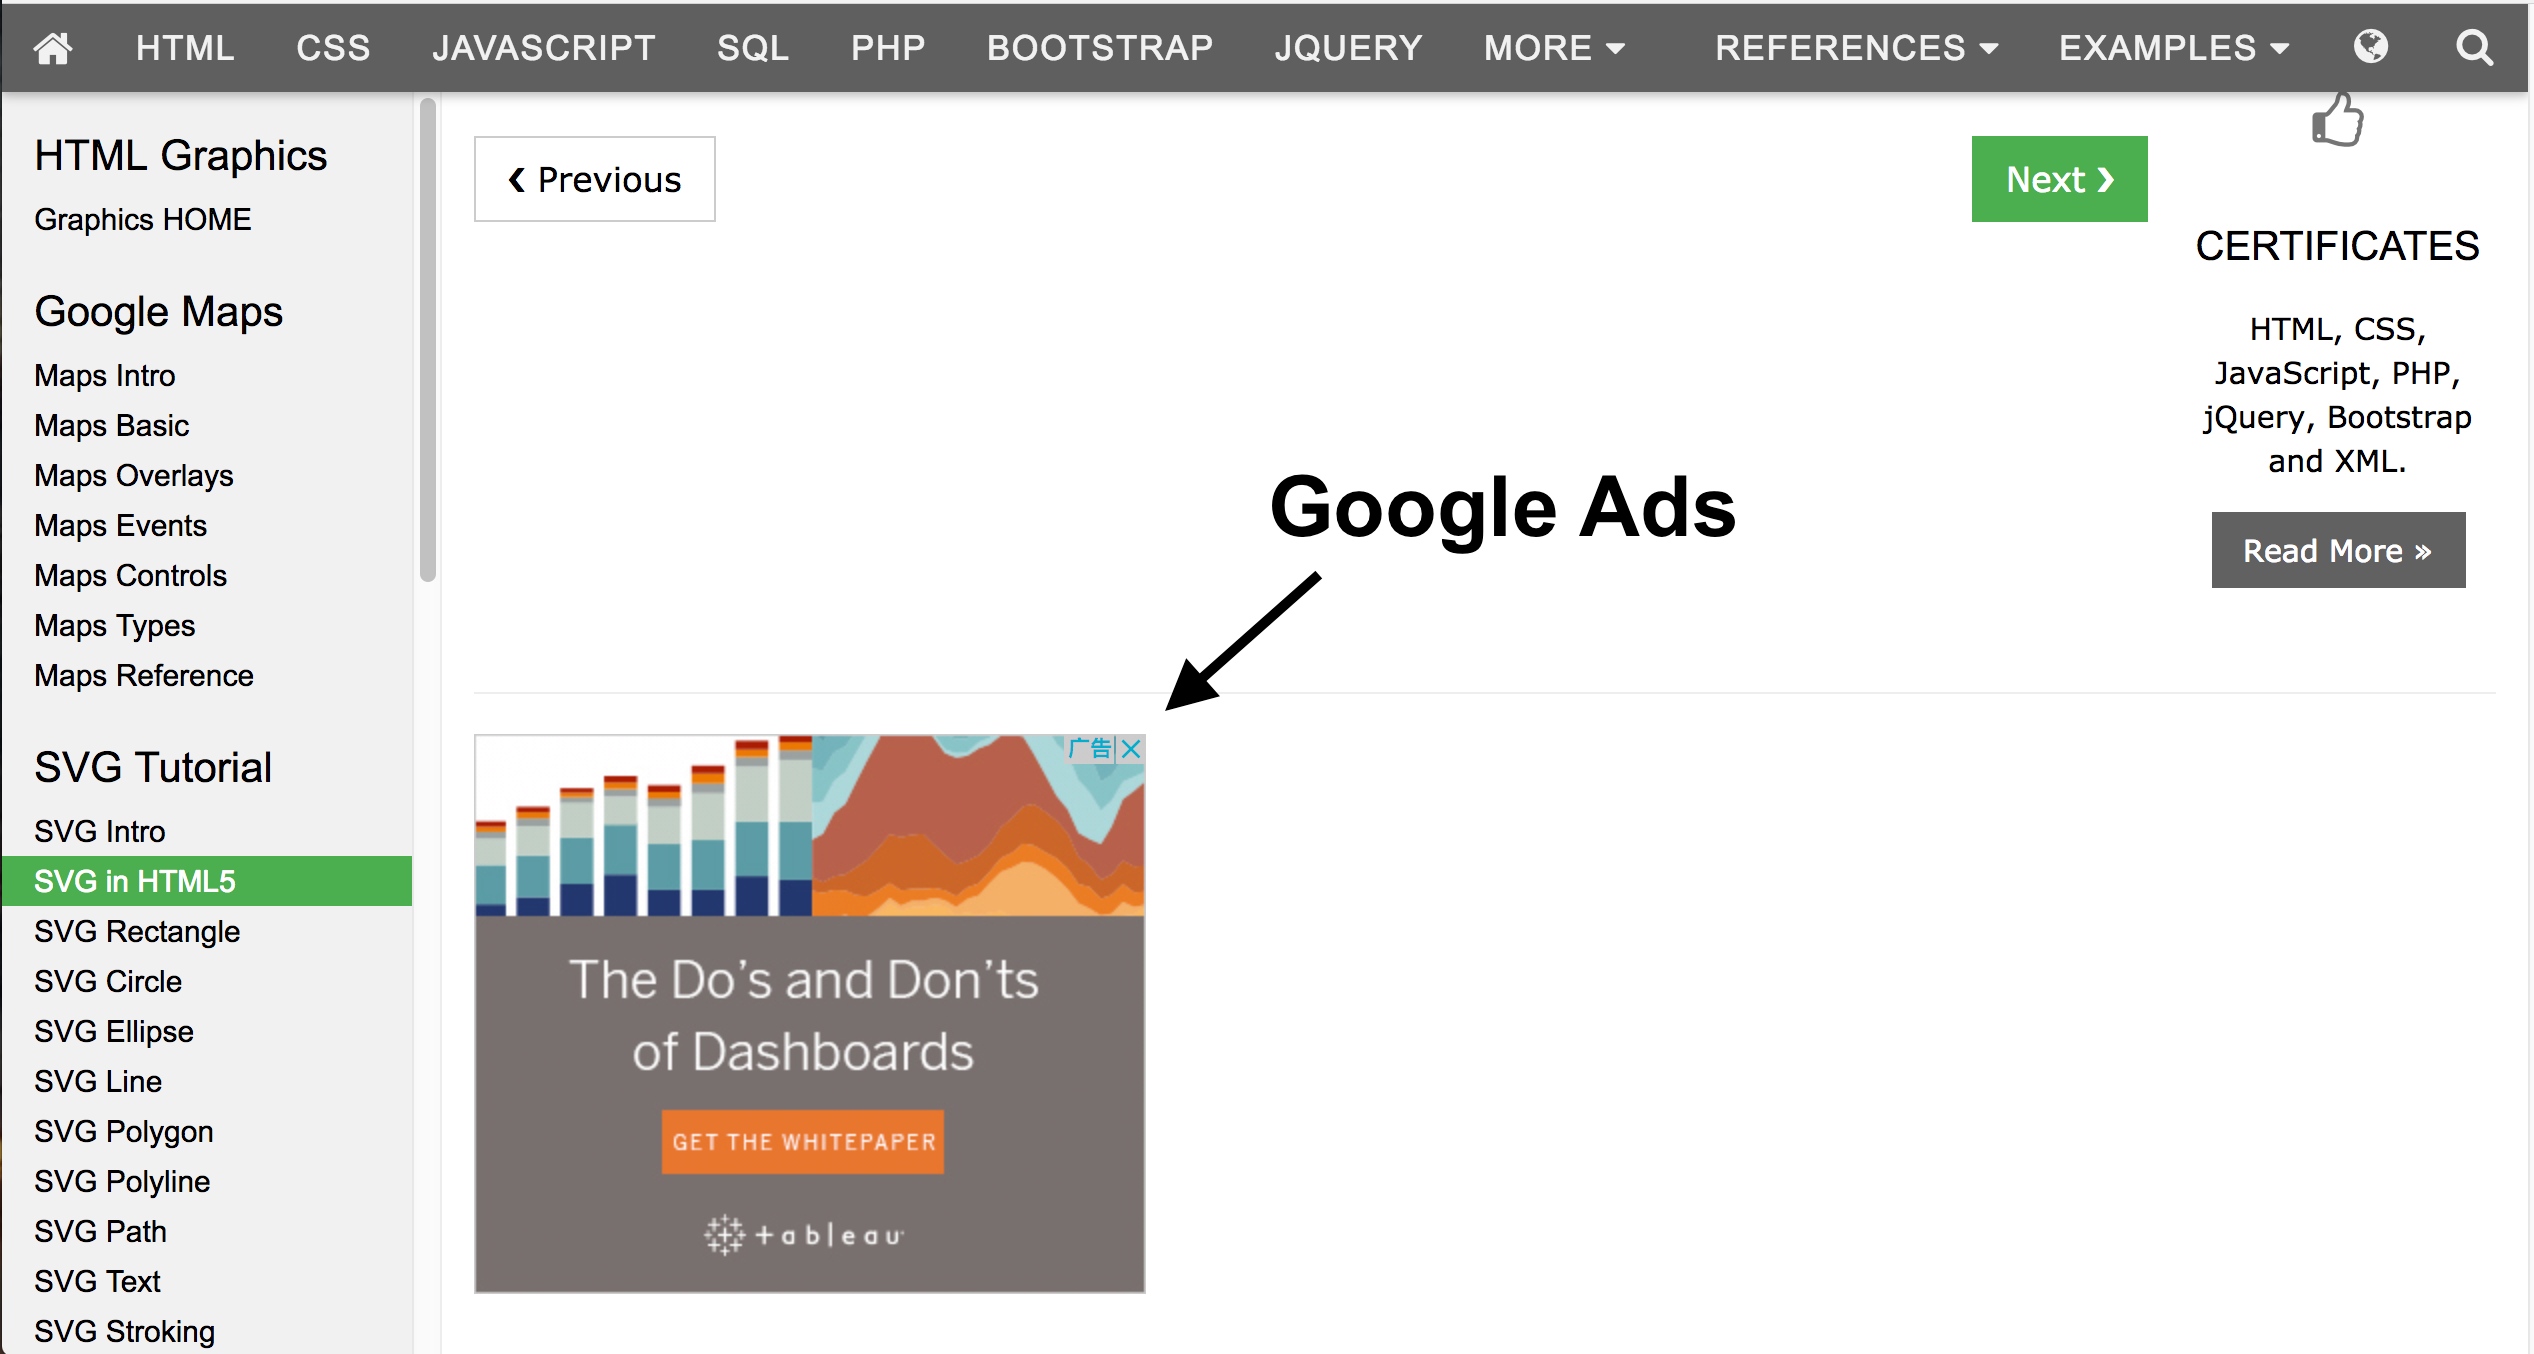
\includegraphics[width=0.5\textwidth]{img/googleAd1}
            \caption{An example of Google Advertisement\cite{googleAd1}}
            \label{img:googleAd1}
        \end{figure}

        \indent
        Behind the advertisement, users can find pages of explanations provided by Google, which tells its users how the recommendation works.
        We can see here in figure \ref{img:googleAd2}. It is the first level of explanations, and Google Ads mainly explains two things here. ``how does it work'' and ``which information is used''.  From the perspective of the first framework - Seven Explanatory Criteria, ``how does it work'' improves the \textbf{transparency}  and increases users' \textbf{trust}, since it exposes the reasoning behind the recommendation to its customers. From the perspective of another framework - Question Type Based Explanation, ``which information is used'' tells users which information Google Ads uses in producing Advertisements. In this way, it can be seen as a \textbf{Input} type question because it explains users which information sources are used to generate the recommendation.
        
        \begin{figure}[H]
            \centering
            \captionsetup{justification=centering}
            \begin{mdframed}
                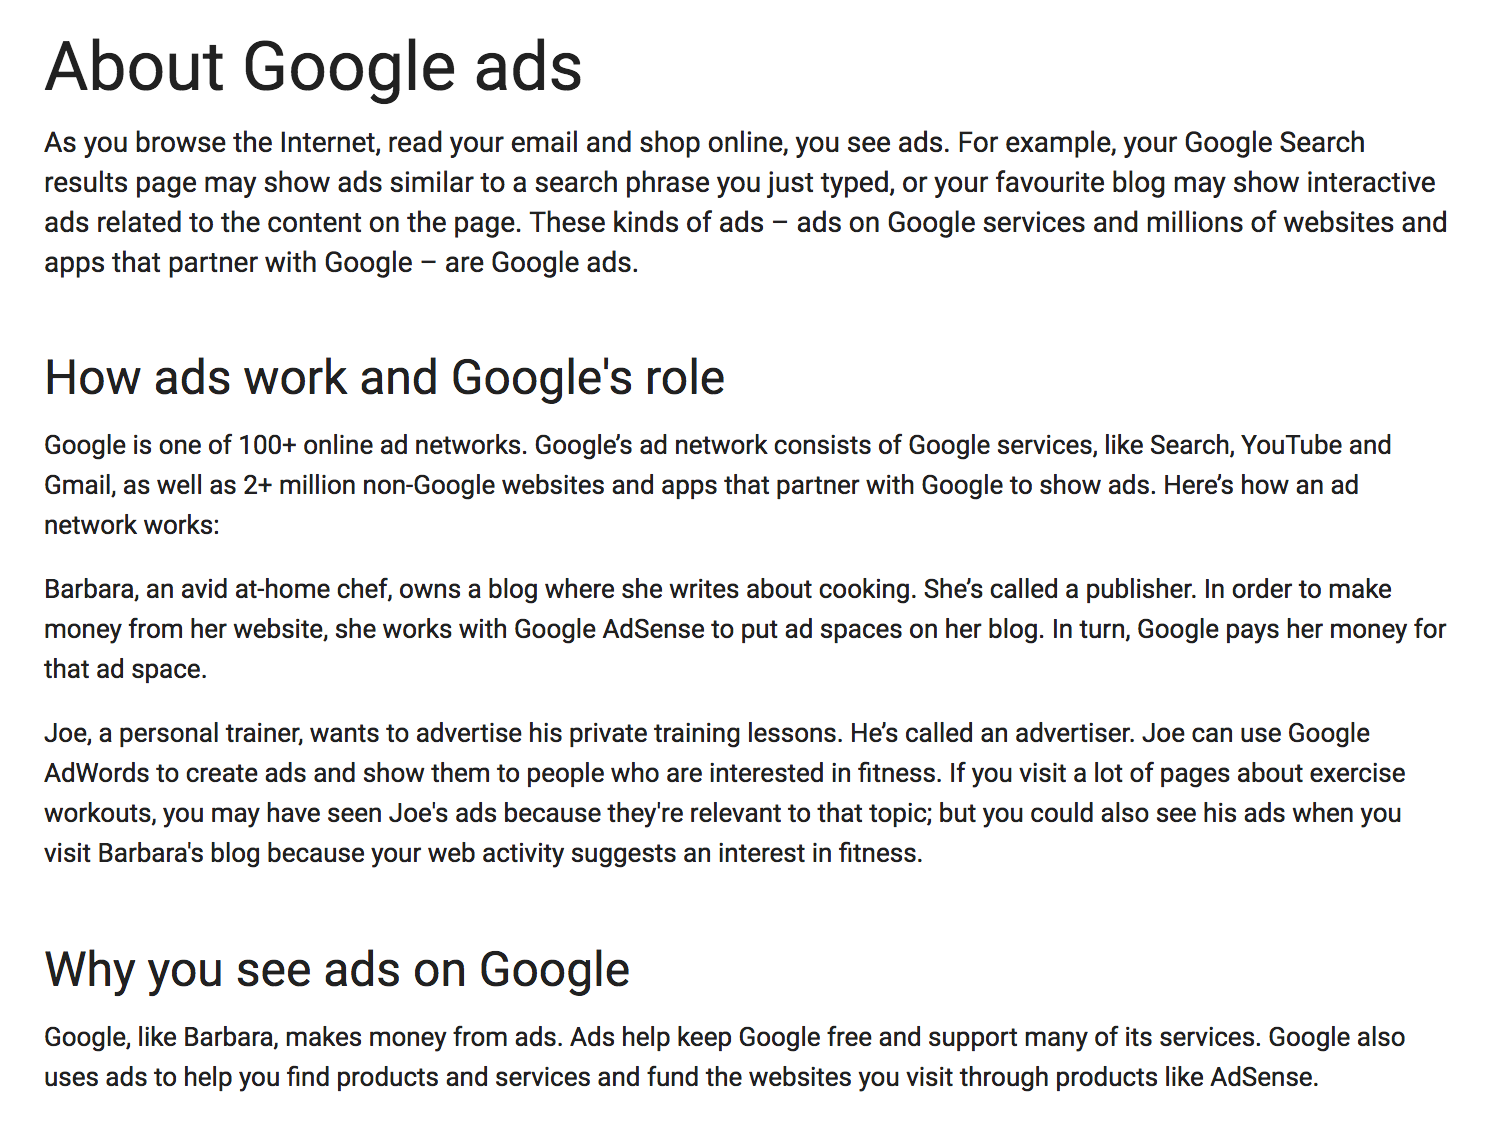
\includegraphics[width=1\textwidth]{img/googleAd2-1}
                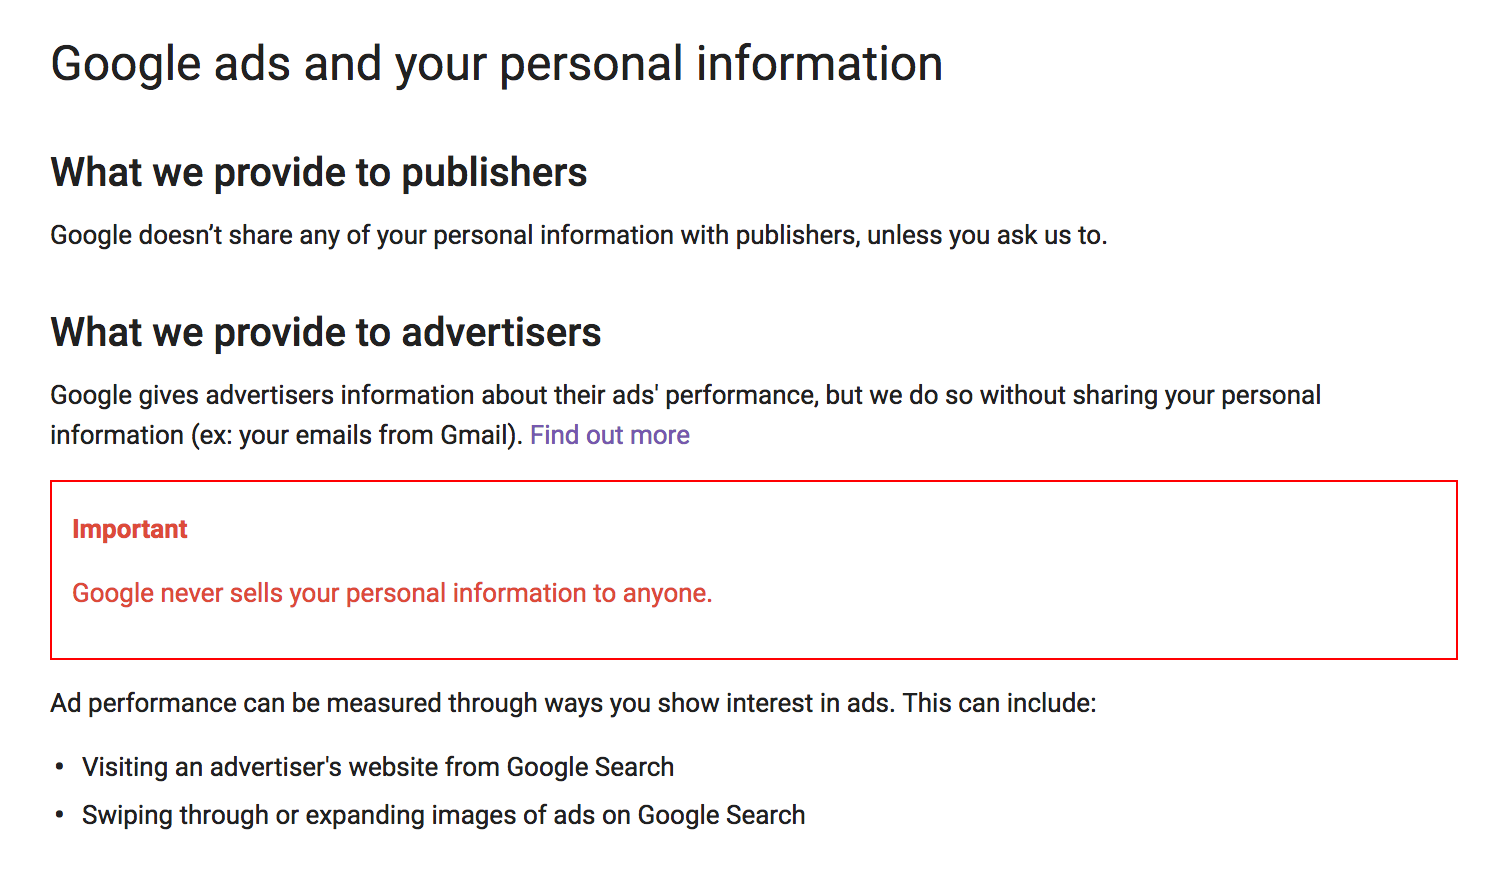
\includegraphics[width=1\textwidth]{img/googleAd2-2}
            \end{mdframed}
            \caption{Explanations from Google Advertisement\cite{googleAd2}}
            \label{img:googleAd2}
        \end{figure}
        \indent
        Figure \ref{img:googleAd3} shows the second level of explanations in Google Ads. It again improves the \textbf{transparency} and increases users' \textbf{trust} in terms of the first framework . Meanwhile, from the perspective of Question-Type-Based explanation, information like, ``You may see ads on Google Search...your location and the time of day'', can be seen as a \textbf{Why} and \textbf{Why Not} question types since they explain the reason why users see certain advertisements.
        \begin{figure}[H]
            \centering
            \captionsetup{justification=centering}
            \begin{mdframed}
                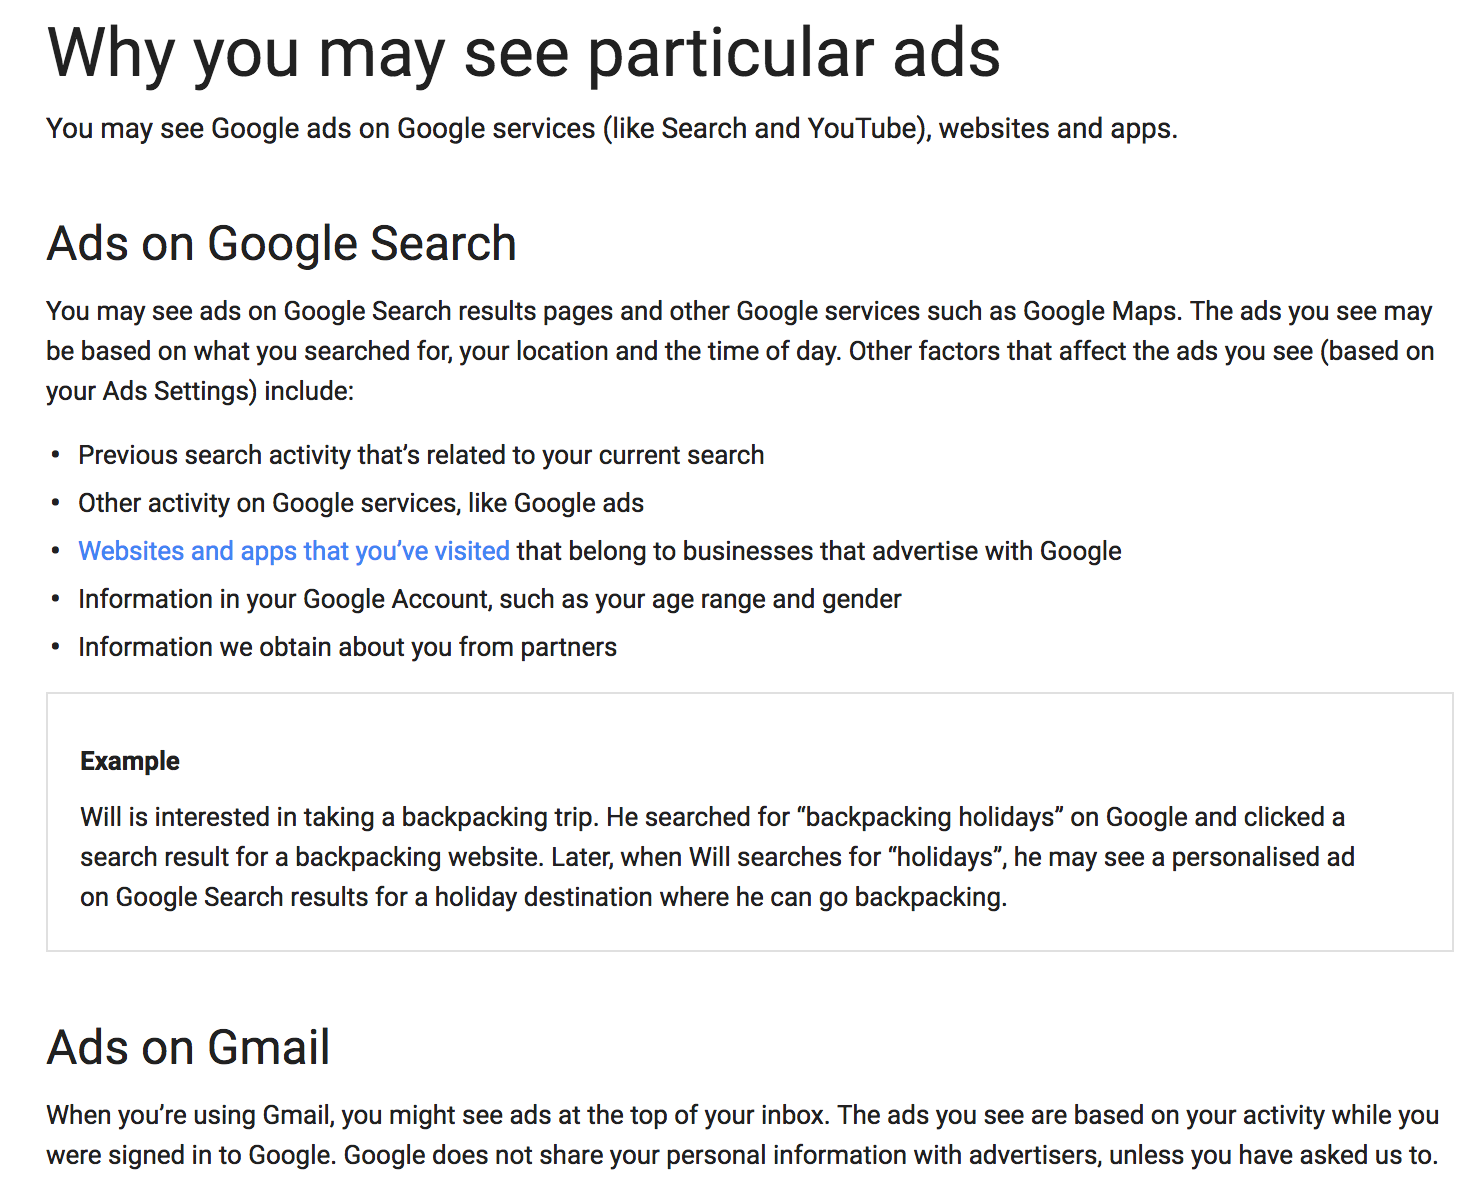
\includegraphics[width=0.8\textwidth]{img/googleAd3-1}
            \end{mdframed}
            \caption{Explanations from Google Advertisement\cite{googleAd3}}
            \label{img:googleAd3}
        \end{figure}
        \begin{figure}[H]
            \centering
            \captionsetup{justification=centering}
            \begin{mdframed}
                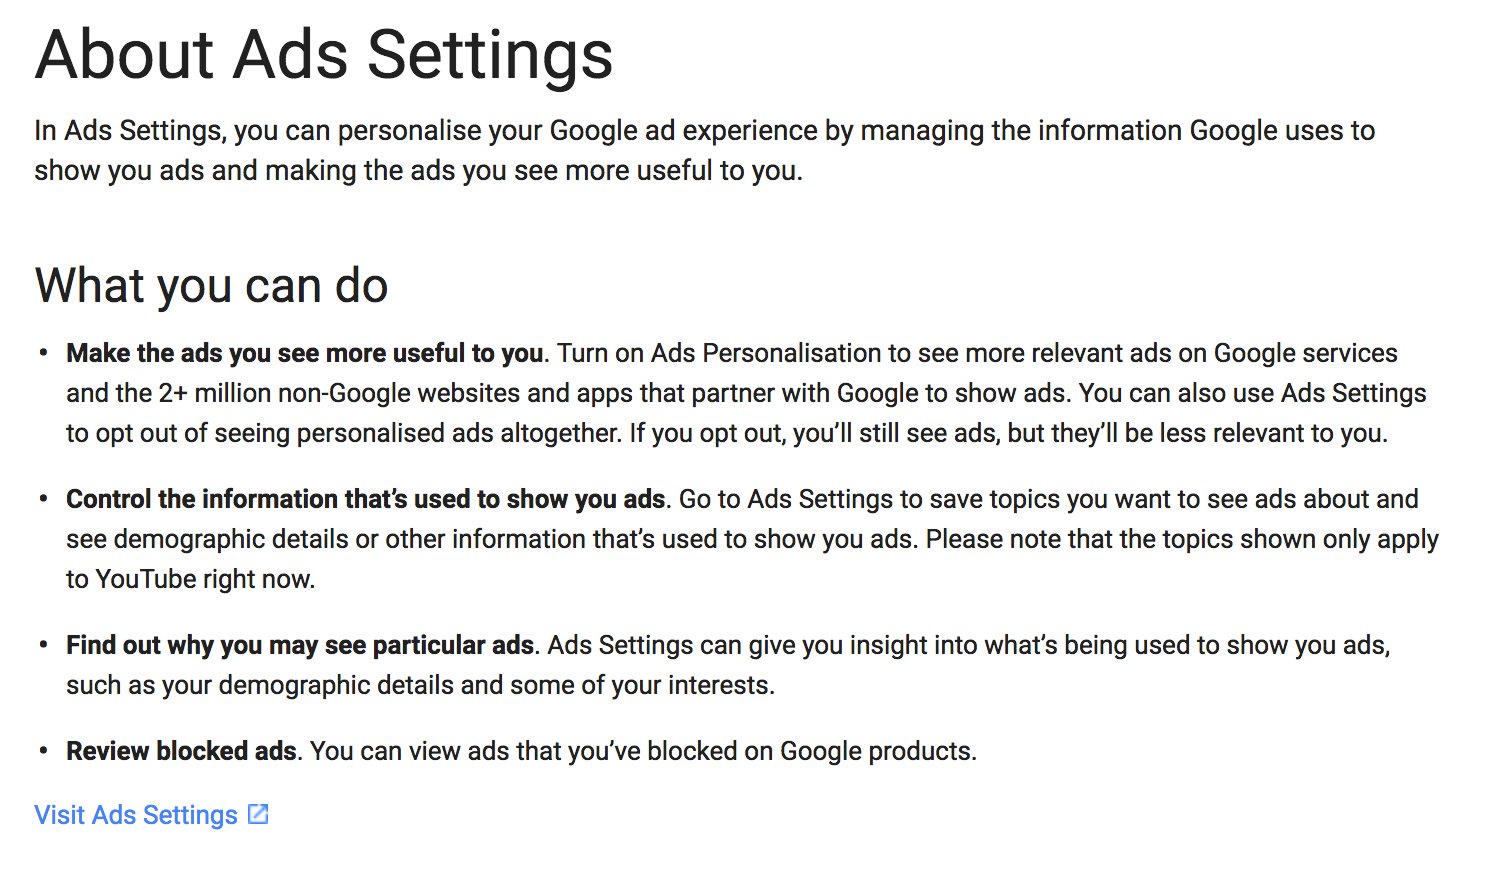
\includegraphics[width=0.8\textwidth]{img/googleAd4-1}
                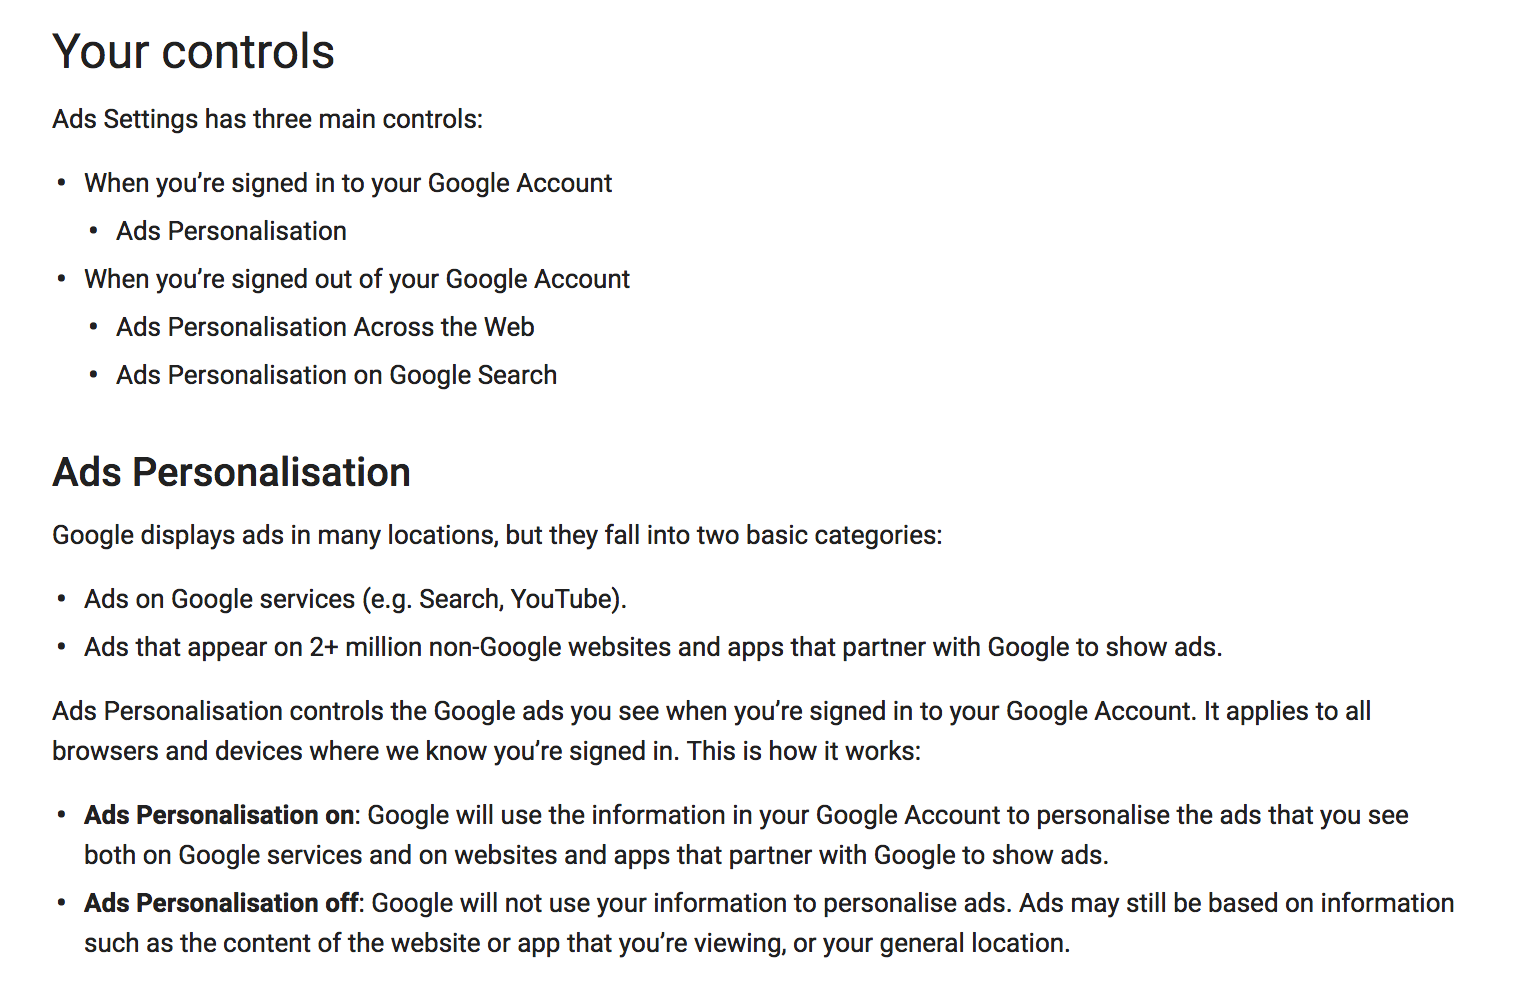
\includegraphics[width=0.8\textwidth]{img/googleAd4-2}
                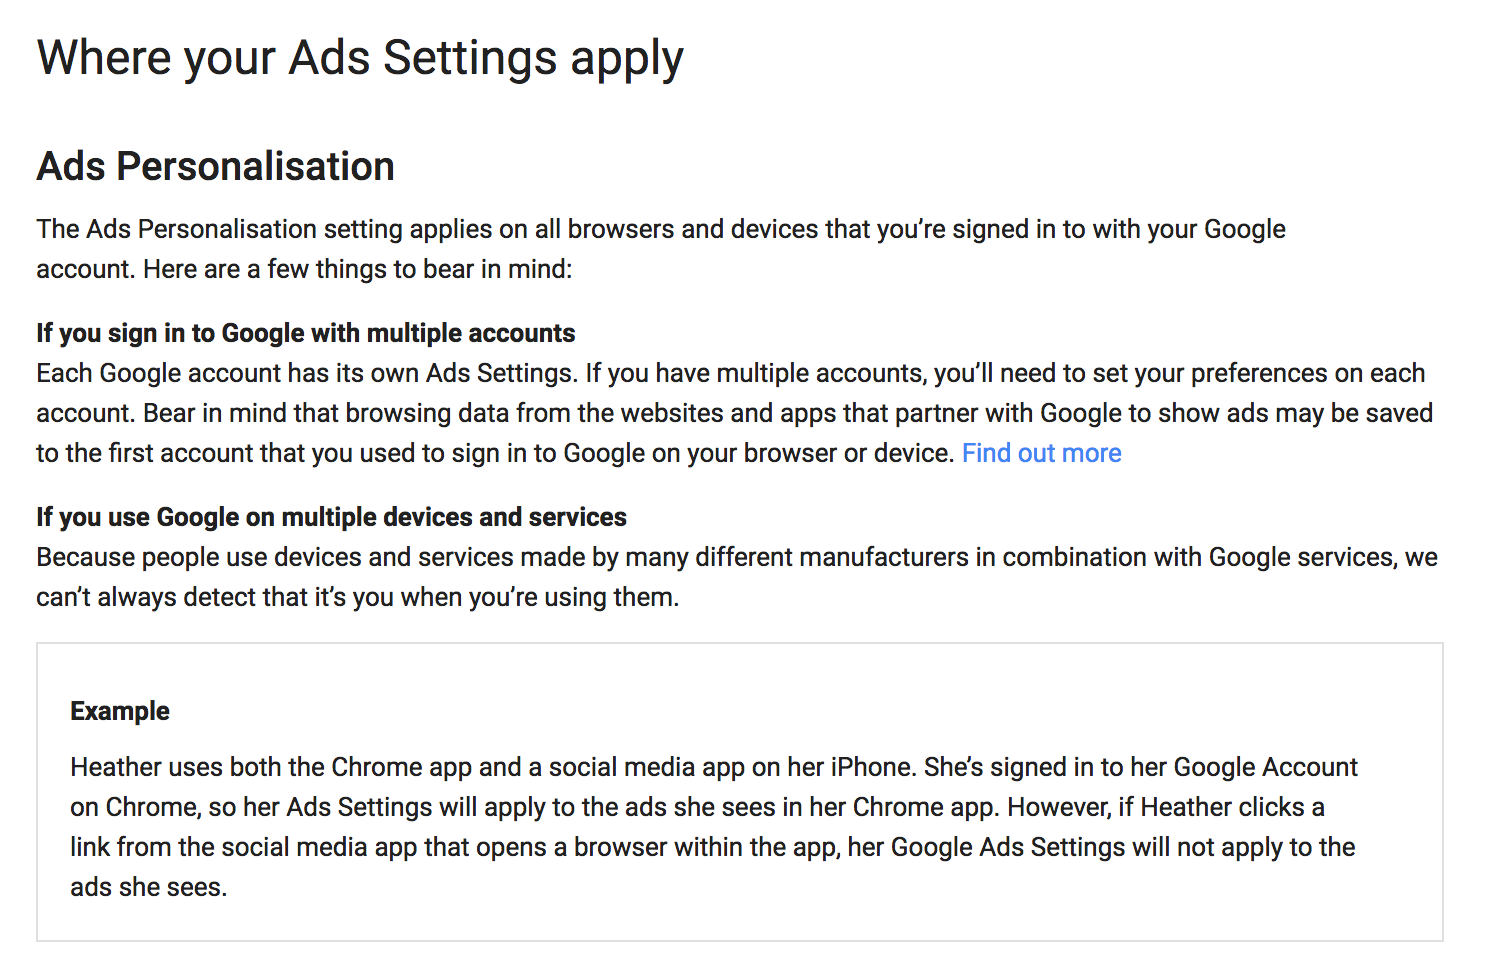
\includegraphics[width=0.8\textwidth]{img/googleAd4-3}
            \end{mdframed}
            \caption{Explanations from Google Advertisement\cite{googleAd4}}
            \label{img:googleAd4}
        \end{figure}
        \indent
        In the next level, Google even allows its users to control their Ads personalization. In figure \ref{img:googleAd4}, explanations are divided into users' authority(``What you can do''), users' controls(``Your controls''), users' ability to turn on/off personalization(``Ads Personalization'') and how to alter the personalization(``Where your Ads settings apply''). From the perspective of Seven Explanatory Criteria again, such accessibility to control the personalisation can be seen as \textbf{Scrutability} since it allows users to avoid the Ads that they are not willing to see. And concerning Question-Type-Based Explanation, it provides users with \textbf{What If} and \textbf{How to}  explanations because it teaches users how to alter their personalisation.
        
        \indent
        Users who care a lot about privacy issues may find explanations of Google Ads helpful because they are transparent and comprehensive. However, it can not match all cases. In some scenarios, like in a driving-context, where brief explanation may be preferred. The next section extracts part of two frameworks mentioned above and tries to figure out which explanation principles fit in with brief explanations.

\section{Brief Explanation}
    \indent In this section, we will dive into brief explanation and introduce how it works in a driving-context and which criteria or factors are helpful when we try to design brief explanation.

    \subsection{Brief Explanation based on Seven Explanatory Criterion}

        \indent Roland Bader and his colleagues used part of Seven Explanatory Criteria and described an automobile assistant system that can reduce driver's distraction while he/she search for some information during driving \cite{bader122011explanations}. The main function of the system is to provide a driver with proactively delivered recommendations. For example, this system can recommend some gas stations to a driver when it detects that the gas level is low. Such proactively delivered recommendations may not be accepted by the driver without a suitable explanation. Thus their goal is to enhance transparency of proactively delivered recommendations by means of explanations and tried to figure out the best way to explain.
    
        \indent In the study, they built the explanations based on \textbf{efficiency} and \textbf{persuasiveness} extracted from the first framework - Seven Explanatory Criteria \cite{bader122011explanations}. The reason why they chose these two principles lies in his application environment. In a driving context, brief explanation may be preferred, and an efficient explanation (efficiency) guarantees short interaction time for decision making, while persuasiveness makes the recommendation convincible (In other words, it persuades the driver that the recommendation right now is relevant to your current state). Roland Bader's and his colleagues then set up a desktop prototype to test users' opinion on their explanations. With each recommendation (like ``The system recommends xxx gas station to you''), explanations are distributed over several levels of detail. The lowest level (first phase), which contains maximal two arguments, like: ``this gas station is on the route or the price of this gas station is low'', provided automatically by the system. Then gradually more and more information can be accessed when the user requests. In the paper, Roland Bader takes the explanations in the lowest level as short explanations \cite{bader122011explanations}.   The first criterion \textbf{persuasiveness} is measured by asking the respondents whether they are satisfied with the explanation (brief explanations) provided in the first phase. And the second criterion \textbf{efficiency} was measured by looking at how often the respondents need to switch to deeper phases with more information.

        \indent The result is as expected. Almost all the experimental respondents were satisfied with the first level explanation, i.e., brief explanation. Besides, they found the information at this stage was adequate for decision-making in normal scenarios, which means that a brief and convincing explanation (persuasiveness) meets users' need. The information in the second level was selected only when particular details were needed, which means that users also prefer an efficient brief explanation (efficiency).

    \subsection{Brief Explanation based on Question-Type-Based-Explanation}
    
    \indent The second framework, Question-Type-Based-Explanation is also a good starting point for designing brief explanations. Based on this framework, Martin Steinert and Larry John Leifer shows how brief explanations of a car’s autonomous action affect the driver’s attitude and safety performance \cite{koo2015did}.

    \indent In their study, two types of information (brief explanation) were provided to explain the auto-braking behavior (car's autonomous action) to the driver during the simulated driving. The first one, ``how'' information, which tells the driver the current state of the car (like: ``the car is braking''), equals to \textbf{``'what'} question type of Question-Type-Based-Explanation in Lim's Toolkit \cite{lim2010toolkit}. The second one is \textbf{``why''} information, which tells the driver the reason why it behaves in certain ways (like: ``Obstacle ahead.'').

    \indent In the user test, they employed a two-by-two between-participants experimental design (see table \ref{table:2}). In table \ref{table:2}, they defined the \textbf{``Why''} type explanation (``Obstacle ahead'') as external information while the \textbf{``What''} type explanation is defined as internal information which describes a car's activity (``The car is braking''). The autonomous action(automatically braking) took place during driving and each time, one of the following four different types of explanations would be presented:
    
    \begin{enumerate}
        \item No explanation.
        \item \textbf{``what''} explanation (``The car is braking'') short before the automatically braking.
        \item \textbf{``why''} explanation (``Obstacle ahead'') short after the automatically braking.
        \item A combination of \textbf{``what''} and \textbf{``why''} explanation(``The car is braking due to obstacle ahead'').
    \end{enumerate}
    \begin{table}[ht] 
        % ht used to attach the table to the position approximately where they are wrote here
        \centering
        \begin{tabular}{ | m{2cm} | m{6em} | m{2cm} | }
        \hline
        %  \bfseries used to bold the header
            & \bfseries Why message & \bfseries without Why message\\ [0.5ex] 
        \hline
        \bfseries what message & Both internal and external information referring to automation & Internal (car activity) information\\ 
        \hline
        \bfseries Without what message & External (situation) information & No information (control condition)\\ 
        \hline
        \end{tabular}
        \caption{Structure of study\cite{koo2015did}}
        \label{table:2}
    \end{table}

    \indent Drivers' attitudes and safety performance were measured in order to learn how different types of information affect the driver. 

    \indent The result shows something different than the original hypothesis. A combination of explanation (\textbf{``why''} + \textbf{``how''}) was supposed to improve driving behaviors. However, the final result indicated that it affected driver attitude negatively. When people were told both how and why the car was about to act on their behalf, they felt anxious. One possible reason for it might be that the driver must process two types of information ( the machine’s status and the situational status) at the same time, which created large cognitive load. Although it was perceived negatively, the combination of explanation (\textbf{``why''} + \textbf{``how''}) contributed to safer driving by minimizing off-lane excursions. 

    \indent With \textbf{``how''} explanation alone, drivers performed the worst: they drifted out of their lane. It seems that drivers felt like they took a passive role in driving if they only received \textbf{``how''} explanation. One possible reason is that human beings expect polite machine behavior \cite{reeves1996people}. Thus, only explaining the car’s behavior, ``Car is braking,'' without explaining the reason might be taken as “impolite.”

    \indent And \textbf{``Why''} explanation alone created the least anxiety and highest trust. This kind of behavior from the system can be seen as transparent, which can, in turn, gain more trust from users. Compared with the combination of explanation (\textbf{``why''} + \textbf{``how''}), the amount of time that it takes to hear and cognitively process the why-only message is shorter, which allowed a quicker response/reaction from the driver. Besides, drivers might find the information valuable and credible when the content satisfies their cognitive need (explain the system's behavior). For this reason, the \textbf{``why''} explanation is more important to drivers and safer because drivers can anticipate upcoming events \cite{koo2015did}.